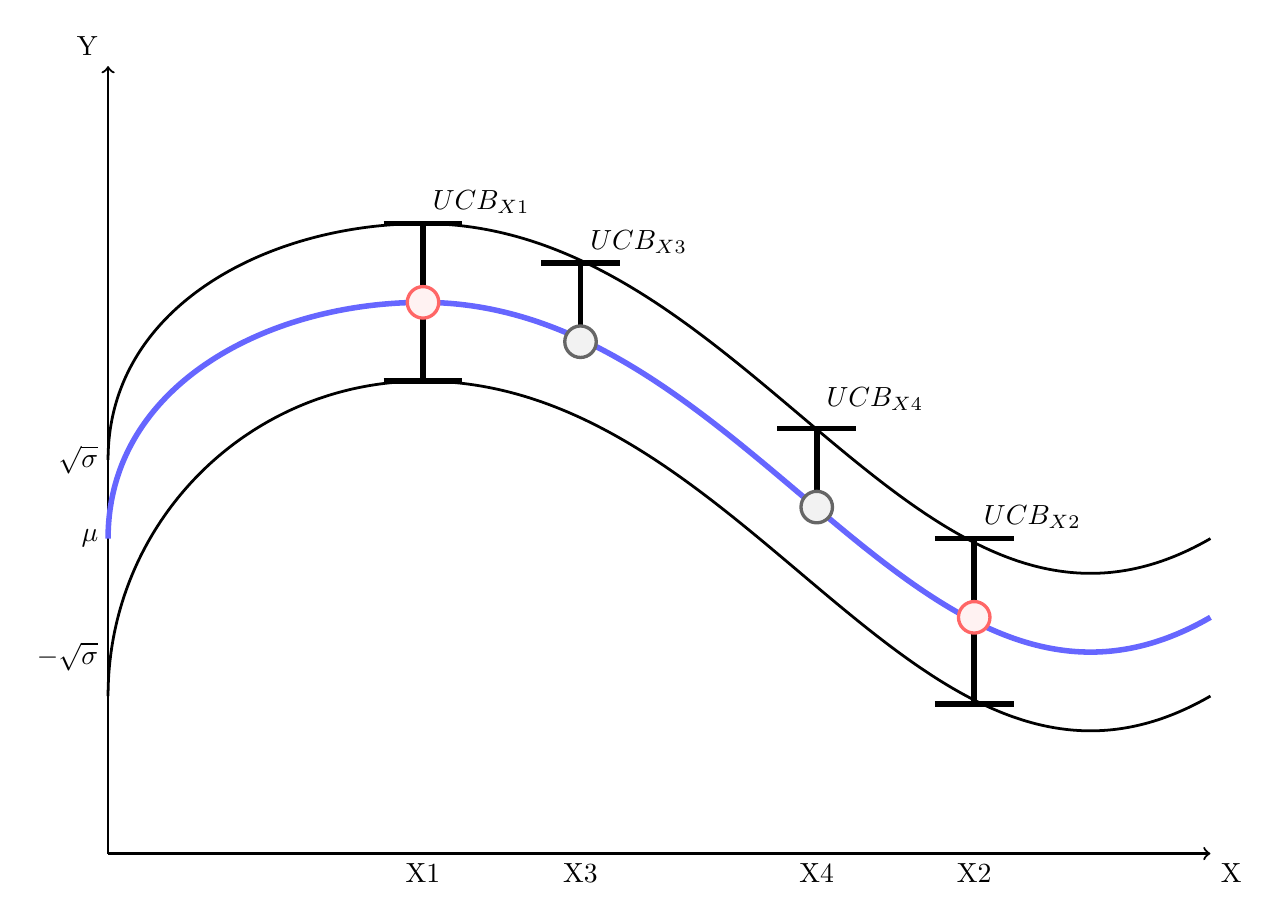
\begin{tikzpicture}


% Draw Axis

\draw[thick,->] (0,0) -- (14,0) node[anchor=north west]{X};
\draw[thick,->] (0,0) -- (0,10) node[anchor=south east]{Y};

% Draw Mean function
\draw[color=blue!60, line width=2pt] (0,4) to [out=90, in=180] (4,7)
to [out=0, in=210] (14,3);

% Draw Lower Bound (-var) function

\draw[line width=1pt] (0,2) to [out=90, in=180] (4,6)
to [out=0, in=210] (14,2);

% Draw Upper Bound (+var) function

\draw[line width=1pt] (0,5) to [out=90, in=180] (4,8)
to [out=0, in=210] (14,4);

% Draw Confidence Interval for X1

\draw[line width = 2pt] (4,6) -- (4,8);

\draw[line width = 2pt] (3.5,6) -- (4.5,6);

\draw[line width = 2pt] (3.5,8) -- (4.5,8);

% Draw X1

\filldraw[color=red!60, fill=red!5, very thick] (4,7) circle (0.2cm);

% Draw Confidence Interval for X2

\draw[line width = 2pt] (11,1.9) -- (11,4);

\draw[line width = 2pt] (10.5,1.9) -- (11.5,1.9);

\draw[line width = 2pt] (10.5,4) -- (11.5,4);

% Draw X4

\filldraw[color=red!60, fill=red!5, very thick] (11,3) circle (0.2cm);

% Draw dashed Confidence Interval for X3

\draw[line width = 2pt] (6,6.5) -- (6,7.5);

\draw[line width = 2pt] (5.5,7.5) -- (6.5,7.5);

% Draw X3

\filldraw[color=black!60, fill=black!5, very thick] (6,6.5) circle (0.2cm);

% Draw dashed Confidence Interval for X4

\draw[line width = 2pt] (9,4.4) -- (9,5.4);

\draw[line width = 2pt] (8.5,5.4) -- (9.5,5.4);

% Draw X4

\filldraw[color=black!60, fill=black!5, very thick] (9,4.4) circle (0.2cm);

% Draw Labels on X-Axis

\node [below] at (4,0) {X1};

\node [below] at (11,0) {X2};

\node [below] at (6,0) {X3};

\node [below] at (9,0) {X4};

% Draw Labels on Y-Axis

\node [left] at (0,4) {$\mu$};

\node [left] at (0,2.5) {$-\sqrt{\sigma}$};

\node [left] at (0,5) {$\sqrt{\sigma}$};

% Draw UCB Labels

\node [above right] at (4,8) {$UCB_{X1}$};

\node [above right] at (11,4) {$UCB_{X2}$};

\node [above right] at (6,7.5) {$UCB_{X3}$};

\node [above right] at (9,5.5) {$UCB_{X4}$};

\end{tikzpicture}